\documentclass{standalone}
\usepackage{tikz}
\usepackage{ctex,siunitx}
\setCJKmainfont{Noto Serif CJK SC}
\usepackage{tkz-euclide}
\usepackage{amsmath}
\usetikzlibrary{patterns, calc,3d}
\usetikzlibrary {decorations.pathmorphing,decorations.pathreplacing,decorations.shapes}
\begin{document}
\small
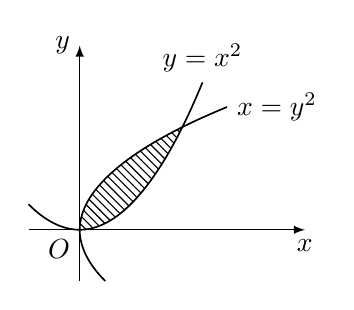
\begin{tikzpicture}[>=latex,scale=1.3]
  \draw[->](-0.5,0)--(2.2,0)node[below]{$x$};
  \draw[->](0,-0.5)--(0,1.8)node[left]{$y$};
  \node at (0,0)[below left]{$O$};
  \draw[semithick](-0.5,0.25)parabola bend (0,0)(1.2,1.44)node[above]{$y=x^2$};
  \draw[semithick,rotate=-90](0.5,0.25)parabola bend (0,0)(-1.2,1.44)node[right]{$x=y^2$};
  \fill[pattern=north west lines](0,0)..controls(1/3,0)and(2/3,1/3)..(1,1)..controls(1/3,2/3)and(0,1/3)..cycle;
\end{tikzpicture}
\end{document}